% !TeX encoding = UTF-8
% !TeX spellcheck = fr_FR

\documentclass{article}
\usepackage[utf8]{inputenc}
\usepackage[french]{babel}
\usepackage[T1]{fontenc}
%====================== PACKAGES ======================
%pour gérer les positionnement d'images
\usepackage{float}
\usepackage{amsmath,amssymb,amsthm}
\usepackage{graphicx}
\usepackage[colorinlistoftodos]{todonotes}
\usepackage{url}
%pour les informations sur un document compilé en PDF et l\section{}es liens externes / internes
\usepackage{hyperref}
%pour la mise en page des tableaux
\usepackage{array}
\usepackage{tabularx}
\usepackage[thinlines]{easytable}
%pour utiliser \floatbarrier
%\usepackage{placeins}
%\usepackage{floatrow}
%espacement entre les lignes
\usepackage{setspace}
%modifier la mise en page de l'abstract
\usepackage{fancyhdr}
\usepackage{abstract}
%police et mise en page (marges) du document

\usepackage{pdfpages}

\usepackage{csquotes}
%Code source
\usepackage{listingsutf8}

\usepackage[top=2cm, bottom=2cm, left=2cm, right=2cm]{geometry}
%Pour les galerie d'images
\usepackage{subfig}

% Glossaire
\usepackage[xindy]{glossaries}	% Ensures that all acronyms are defined once
\makeglossaries

\pagestyle{fancy}
\headheight=14.62pt

%% Mise en page des théorèmes, lemme etc...
\theoremstyle{plain}
\newtheorem{thm}{Théorème}[section]
\newtheorem{lemme}[thm]{Lemme}
\newtheorem{prop}[thm]{Proposition}
\newtheorem*{cor}{Corollaire}
\theoremstyle{definition}
\newtheorem{defn}{Définition}[section]
\newtheorem{conj}{Conjecture}[section]
\newtheorem{exmp}{Exemple}[section]
\theoremstyle{remark}
\newtheorem*{rem}{Remarque}
\newtheorem*{note}{Note}
\newtheorem{case}{Cas particulier}

\renewcommand{\floatpagefraction}{0.95}
\renewcommand{\textfraction}{0.05}

\addbibresource{biblio.bib}

%====================== INFORMATION PDF======================

\hypersetup{												% Information sur le document
	pdfauthor = {Fati CHEN},								% Auteurs
	pdftitle = {Ouvertures et Finales d'Eternity II},		% Titre du document
	pdfsubject = {Rapport de Projet},						% Sujet
	pdfkeywords = {Eternity II, rapport de projet, LIRMM},	% Mots-clefs
	pdfstartview={FitH}										% ajuste la page à la largueur de l'écran
	pdfcreator = {MikTeX},									% Logiciel qui a crée le document
	pdfproducer = {Eternithug}}								% Société avec produit le logiciel


%======================== DEBUT DU DOCUMENT ========================
\begin{document}

	%__ Listes
	\renewcommand{\labelitemi}{$\bullet$}
	\renewcommand{\labelitemii}{$\--$}
	\renewcommand{\labelitemiii}{$\diamond$}
	\renewcommand{\labelitemiv}{$\ast$}

	%__ régler l'espacement entre les lignes
	\newcommand{\HRule}{\rule{\linewidth}{0.5mm}}

	%========================= Debut du texte =========================

	\pagenumbering{Alph}

\begin{titlepage}
	\begin{center}
	
	% Upper part of the page. The '~' is needed because only works if a paragraph has started.
	%\includegraphics[width=0.35\textwidth]{./logo}~\\[1cm]
	
	\textsc{\LARGE Faculté des Sciences\\
		Université de Montpellier\\
		Lirmm\\} \ \\[1.5cm]
	
	\textsc{\Large }\\[0.5cm]
	
	% Title
	\HRule \\[0.4cm]
	
	{\huge \bfseries Rapport de stage\\
	Ouvertures et finales d'Eternity II\\[0.4cm] }
	
	\HRule \\[1.5cm]
	
	% Author and supervisor
	\begin{minipage}{0.4\textwidth}
		\begin{flushleft} \large
			\emph{Auteurs:}\\
				Fati \textsc{Chen}\\
		\end{flushleft}
	\end{minipage}
	\begin{minipage}{0.4\textwidth}
		\begin{flushright} \large
			\emph{Référent:} \\
				Eric \textsc{Bourreau}
		\end{flushright}
	\end{minipage}
	
	\vfill
	\thispagestyle{empty}

	% Bottom of the page
	{\large \today}
	\end{center}
\end{titlepage}

\pagenumbering{arabic}
	\newpage

	\thispagestyle{empty}
	\null
	\newpage
	
	\setcounter{page}{1}
	% Table des matières
	\tableofcontents
	\newpage
	
	% Table des figurs 
	\listoffigures
	\newpage
	
	\listoftables
	\newpage
	\thispagestyle{empty}
	\section*{Remerciements}
	Je tiens tout d'abord à remercier Eric BOURREAU, mon encadrant pour m'avoir proposé ce stage, je tiens évidemment à remercier le LIRMM et l'UM pour l'accueil et l'hospitalité. 
	
	Je remercie aussi toute l'équipe MAORE,la ribambelle de stagiaire et toutes les autres personnes dont j'ai fait la connaissance durant ces deux courts mois. Grâce à eux j'ai découvert de nouvelles choses.
	
	Enfin, je remercie ma famille et mes amis pour leur aide, leur intérêt et leur soutien, notamment Raphaël, Anthony et Jean--François qui m'ont aidé, entre autres, à la relecture de ce rapport.
	\newpage

	\section{Introduction}

	Les puzzles et casses-têtes nous ont toujours passionnés, pour faire passer le temps ou pour se poser des défis. Eternity II est un de ces jeux où le principe peut être compris par tous, mais pourtant sa résolution est extrêmement complexe. Ce genre de paradigme est à l'heure actuelle l'un des problèmes mathématiques qui régissent notre monde. La plupart des systèmes informatiques et méthodes de chiffrement reposent sur ce genre de mécanisme : une simplicité de mise en place, mais une complexité de destruction.

	Eternity II n'est solvable à l'heure actuelle qu'en testant toutes les combinaisons par méthode de bruteforce. Ce qui nous fait poser une question importante : comment, avec l'augmentation exponentielle des données et des nouvelles technologies, sommes-nous réduit à utiliser une méthode aussi simple. Par extension, est-il plus efficace d'accumuler des données avant de le résoudre plutôt qu'essayer d'accélérer la résolution basique.

	Dans un premier temps, nous verrons les origines du jeu, la difficulté à laquelle nous sommes confrontés et l'état de l'art des méthodes de résolution.
	
	Ensuite, nous présenterons la problématique, ce qui à déjà été fait tout au long de l'année et l'approche initiale du problème.
	
	Pour conclure, nous évoquerons les résultats et réflexions qui peuvent en être tirés.
	
	Par ailleurs, ce compte rendu comporte un manuel d'utilisation et un manuel technique fourni, car les applications développées, ou tout du moins leur logique, est destinée à être réutilisée ou améliorée.


	\newpage
	% !TeX root = main.tex
\section{Eternity II}
	\subsection{Les origines}
	--- [réel]
	
	Eternity II est le fier successeur de Eternity.
	
	La première version sortie en 1999, était composée de 159 pièces de différentes formes, cependant ces formes peuvent être décomposés en formes de trianges equilatéraux (ou leur moitié) qui devaient être placés sur un plateau octogonal. 
	
	\begin{figure}[H]
		\minipage{0.65\textwidth}
		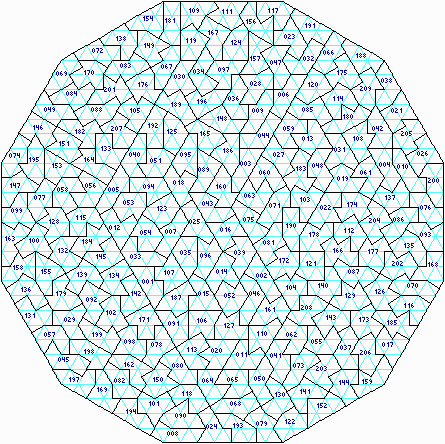
\includegraphics[width=\linewidth]{images/eternity_1.jpg}
		\caption{Eternity I}\label{fig:eternity_1}
		\endminipage\hfill
		\minipage{0.33\textwidth}
		
\includegraphics[width=\linewidth]{images/eternity_1_piece.jpg}
		\caption{Forme d'une pièce d'EternityI}\label{fig:eternity_1_piece}
		\endminipage\hfill
	\end{figure}

	Son point faible se trouvaient dans la disposition de ces pièces sur le plateau : il était possible de précalculer des régions, puis de les comparer entre eux afin d'en dégager une solution.
	De cette facon, le puzzle fut résolu en à peine un an (contrairement aux 3 ans prévus par le créateur), par deux mathématiciens, qui ont ainsi empoché la récompense s'élevant à $1000000\pounds$.
	
	Après cet \enquote{echec}, Christopher Monckton, le créateur d'Eternity, décide en 2008 de sortir une deuxième version, bien plus complexe avec à la clé $2000000$\textdollar pour celui qui arriverait à la résoudre au bout de deux ans.
	
	\begin{figure}[H]
		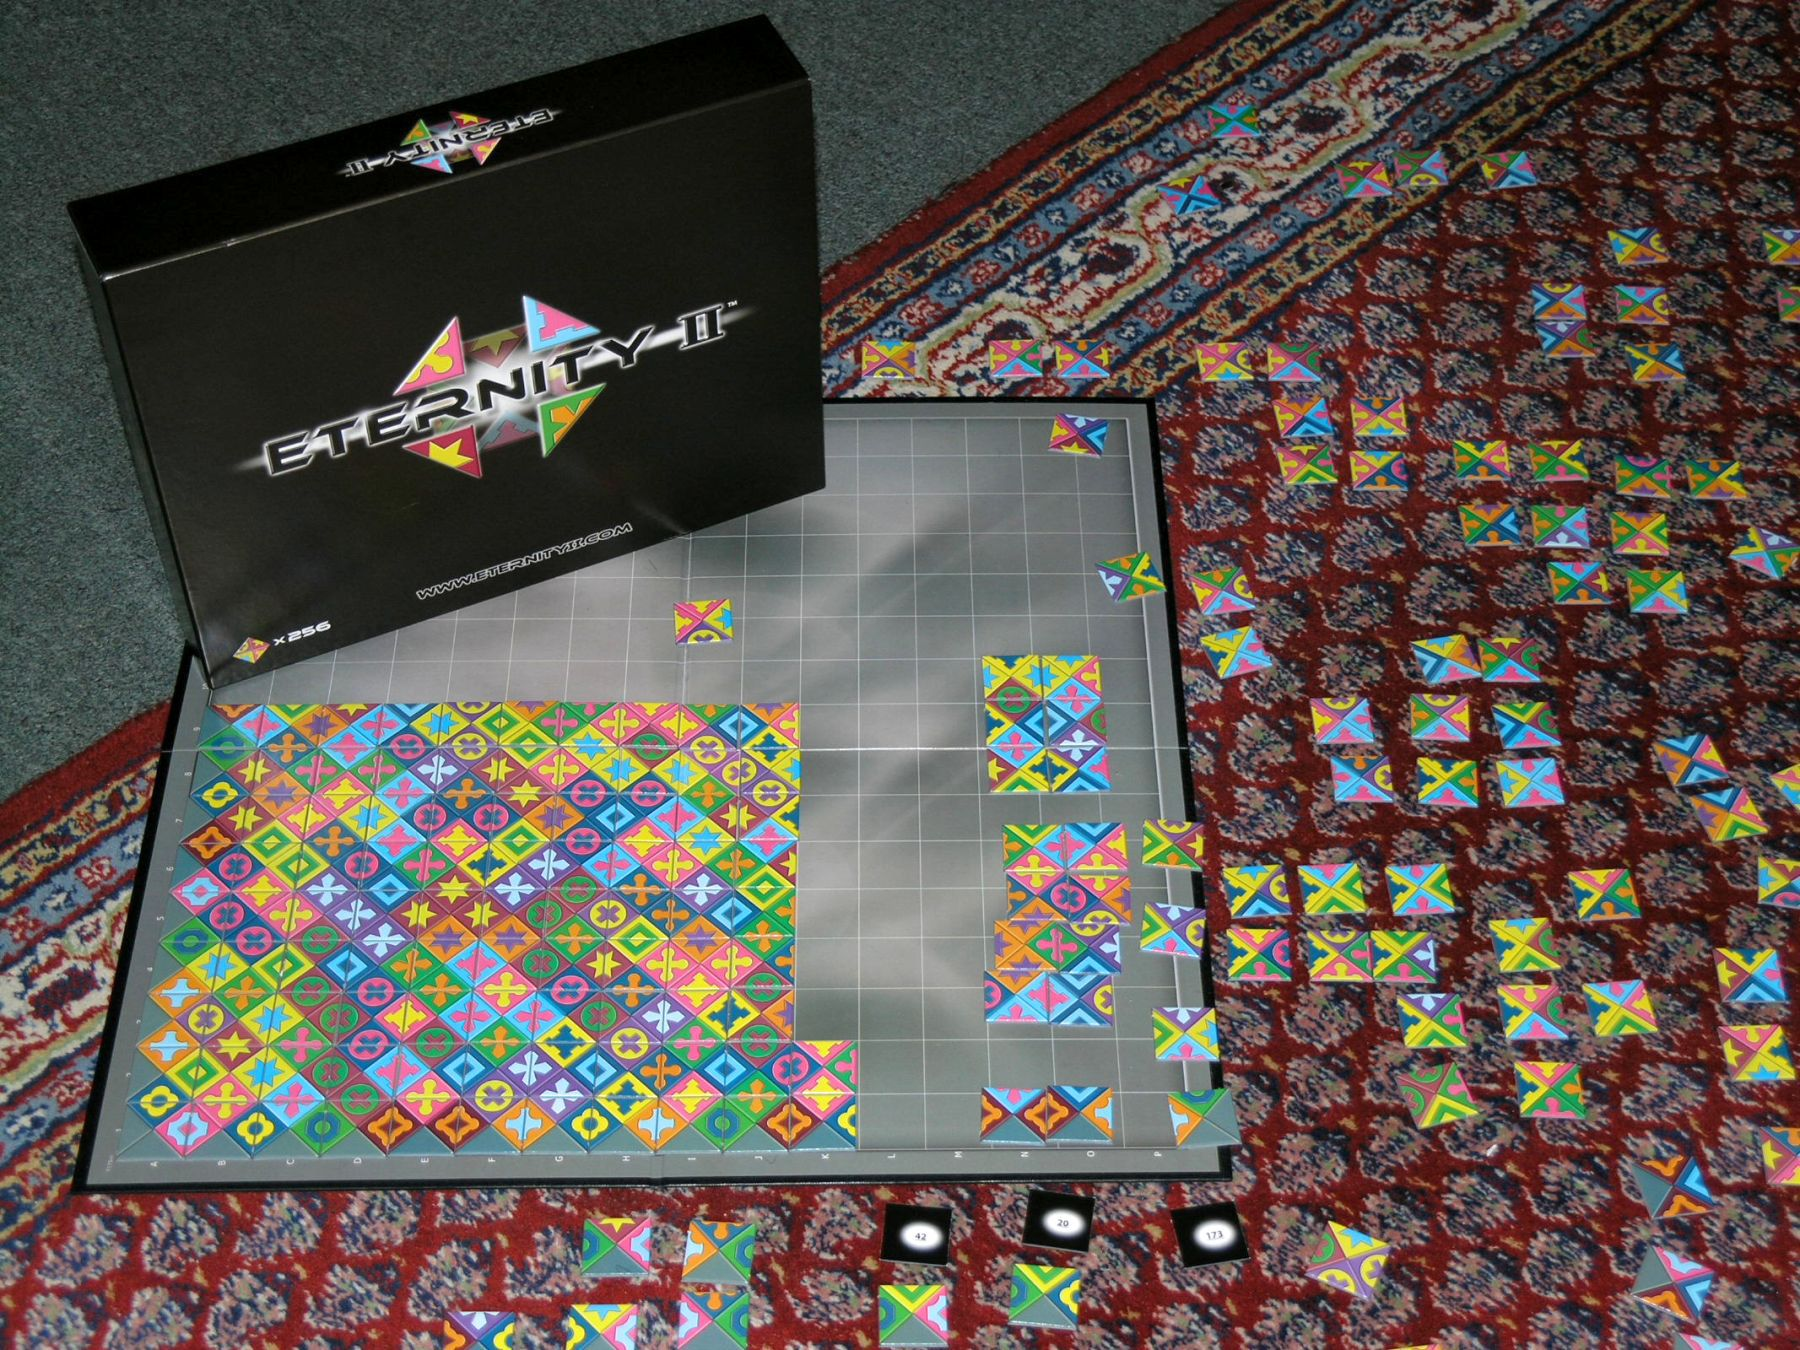
\includegraphics[width=\linewidth]{images/eternity_2.jpg}
		\caption{La boite et les pièces d'Eternity II}
		\label{fig:eternity_2}
	\end{figure}
	
	C'est un puzzle de 16 par 16 qui sort sous le nom d'Eternity II. Ce puzzle est composé de 256 pièces carrés, qui ont chacune 4 faces colorés (ou un demi motif).
	
	Ces pièces peuvent être classés en trois catégories suivant le nombre de faces grises qu'elles possèdent :
	
	\begin{figure}[H]
	   	\minipage{0.32\textwidth}
	   	
\includegraphics[width=\linewidth]{images/piece_coin.png}
	   	\caption{\textbf{pièce de coin :} 2 faces grises}\label{fig:piece_coin}
	   	\endminipage\hfill
	   	\minipage{0.32\textwidth}
	   	
\includegraphics[width=\linewidth]{images/piece_bord.png}
	   	\caption{\textbf{pièce de bord :} 1 faces grise}\label{fig:piece_bord}
	   	\endminipage\hfill
	   	\minipage{0.32\textwidth}
	   	
\includegraphics[width=\linewidth]{images/piece_interieure.png}
	   	\caption{\textbf{pièce d'intérieur :} toutes les faces de couleur}\label{fig:piece_interieure}
	   	\endminipage
	\end{figure}

	Les pièces ne possèdent pas de formes comme dans un puzzle classique. Afin de les faire correspondre l'une avec l'autre, il est nécessaire que les faces adjacentes de chaque pièce voisine soient de la même couleur, dés lors les pièces \enquote{matchent} \ref{fig:matching}.
	
	\begin{figure}[H]
		\centering
		
\includegraphics{images/matching_pieces.png}
		\caption{Deux pièces correctement placés (matchés)}\label{fig:matching}
	\end{figure}
	
	Par conséquent, une pièce peut quasiment être placée n'importe où sur le plateau car son placement dépend des couleurs des pièces d'à côté, de plus, les pièces n'ont pas d'orientation prédéterminés (elles peuvent être rotationnée).
	
	Pour résumer, la plupart des pièces peuvent être posés n'importe où sur le plateau à différentes rotation car la position dépends entièrement des pièces adjacentes posés auparavant. 
	
	Enfin, comme leur nom l'indiquent, les pièces de coins sont les seules à pouvoir être posés dans les coins du plateau, c'est aussi valable pour les pièces de bord qui ne peuvent être placés que sur les bords du plateau, ces deux types de pièces ne peuvent pas être ailleurs car leurs faces grises doit \enquote{matcher} avec les bords du plateau.
	
	
	--- [résumé]
	
	Eternity II est un jeu sorti en 2008 qui repose sur un principe assez simple, c'est un puzzle de 16 par 16 qu'il faut réassembler. Il est composé de 256 pièces carrés, qui ont, sur chaque arête une couleur donnée. [images tt ca tt ca]. Afin de pouvoir assembler le puzzle, il suffit placer les pièces de façon à ce que les faces adjacentes soient de même couleur. Comme un puzzle classique, il y a des pièces de coin et de bord. Ceux-ci sont reconnaissables car ils possèdent une ou deux arêtes grises. Par contre, la où ca devient complexe, c'est qu'une pièce n'as pas une place prédéterminée (comme dans un puzzle), c'est à dire qu'elle peux se situer n'importe où sur le plateau. 
	
	\newpage
	\subsection{Le défi}
	--- [réel]
	
	Malgré le fait que la récompense à expiré le 31 décembre de l'année 2010, le problème et l'enthousiasme qu'a engendré Eternity II ne c'est pas calmé pour autant (enfin si\dots un peu). Car loin d'être juste un jeu avec une importante cagnotte il recel en son c\oe ur des secrets d'une certaine valeur.
	
	En effet, jusqu'à maintenant, personne n'a réussi à résoudre ce puzzle, même pas effleuré la solution, malgré l'aide de supercalculateurs et de nombreux spécialistes, que ce soient des mathématiciens ou des informaticiens.
	
	Pourquoi ? Car derrière ce jeu anodin se cache l'un des plus grand problème du monde actuel : les problèmes NP-difficiles. Ceux-ci sont fait de telle sorte que même ne connaissant leur structure ou fonctionnement, il est pratiquement impossible d'en déduire un algorithme (moyen de résoudre) afin de trouver la solution. Ce type de problème est communément appliqué dans le chiffrement. Car le meilleur moyen de cacher une aiguille (solution) est de la cacher dans gros paquet d'aiguilles, plus le tas est gros, plus on met de temps à la [l'aiguille] trouver.
	
	\begin{exmp}
		Le nombre de combinaisons possibles pour Eternity II s'élève à $10^{545}$, c'est à dire environ $10^{450}$ fois le nombre d'atomes dans l'univers connu (estimé à au plus $10^{80}$) !!! Ca fait un gros tas d'aiguilles !!
	\end{exmp}
		
	--- [résumé]
	
	A ce jour, personne n'a réussi à résoudre ce puzzle (même grâce à l'aide de supercalculateurs) malgré les différentes stratégies mise en place. Pourquoi ? Car derrière ce jeu anodin se cache l'un des plus grand problème du monde actuel : les problèmes NP-difficiles. Ceux-ci sont fait de tel sorte que même en connaissant leur structure ou fonctionnement, il est pratiquement impossible d'en déduire un algorithme de résolution. L'une des solutions les plus fiables à ce jour est de tester tout les cas possible (qui est évidemment très important).
	
	\begin{exmp}
		Le nombre de combinaisons pour Eternity II s'élève à $10^{545}$, c'est à dire environ $10^{450}$ fois le nombre d'atomes dans l'univers connu (estimé à au plus $10^{80}$) !!!
	\end{exmp}
	
	\subsection{Les II lois d'Eternity II}
	
	--- [réel]
	
	Pour rendre Eternity II complexe et combinatoire, il est nécessaire de respecter les deux lois d'Eternity II :
	
	\begin{law}
		\textbf{Chaque pièce est unique}
		
		L'unicité des pièces est indispensable pour complexifier le problème, car sinon, on peux considérer qu'une pièce peux être placée à plusieurs endroits, en fonction du nombre de \enquote{clones} qu'elle possède. Ce qui réduit grandement l'espace de recherche [de la solution].
	\end{law}

	\begin{law}
		\textbf{La quantité de couleurs et de pièces est finement calculée}
		
		En effet, si l'on augmente le nombre de couleurs, on obtient des couplage uniques : une pièce ne peux être couplée qu'avec une autre pièce (ou dans le meilleur des cas limite le couplage des pièces). A l'inverse, si il n'y a pas assez de couleurs, on obtient des doublons, les pièces ne sont plus uniques, ce qui va à l'encontre de la première loi.
		
		Par ailleurs, certaines couleurs sont exclusives aux pièces de coin et de bord, car ceux-ci étant liés en eux mais seulement sur le périmètre extérieur du plateau il est nécessaire d'ajouter des couleurs supplémentaires tenant compte qu'ils n'ont que 2 ou 3 faces disponibles (le reste étant des faces grises).
	\end{law}
	
	
	--- [résumé]
	
	Pour rendre ce problème combinatoire, il est nécessaire de respecter plusieurs conditions.
	
	\begin{description}
		\item[Chaque pièce est unique] l'unicité des pièces est importante, car si une pièce est en double, cela veux dire que la pièce peux être placée à deux endroits différents (ce qui simplifie le problème)
		\item[Le ratio de nombre de couleurs par nombre de pièces est calculé] [joindre graphique tt ca tt ca] : il faut qu'il y ait assez de couleur pour que chaque pièce soit unique, mais pas assez pour que l'on puisse déterminer les pièces adjacentes
		
		\begin{exmp}
			Supposons qu'il y ait trop de couleurs. Cela veux dire qu'une pièce à peu de voisins ( car chaque pièce est unique, par conséquent les couleurs sont distribués uniformément à travers les pièces), si la pièce à très peu de voisins, je peux déduire des groupement de pièces assez facilement.
			
			Donc je simplifie mon problème.
		\end{exmp}		
	\end{description}
	
	\subsection{Etat de l'art}
	
	Un grand nombre de méthodes ont été mis en place afin de résoudre ce problème.
	
	Il serait trop long de présenter et décrire les différents méthodes mise en place car il requièrent une certaine connaissance dans les domaines auxquels ils sont appliqués. Malgré tout, Les différentes approches seront notés ici à titre informatif.
	
	Pour commencer, il existe plusieurs solveurs graphiques afin de pouvoir résoudre le puzzle manuellement ou assisté par l'ordinateur. Certains d'entre eux permettent même l'import export de la progression actuelle.
	
	\begin{itemize}
		\item E2\_manual : \url{https://sourceforge.net/projects/e2manual/}(anglais)
		\item E2Lab : \url{http://eternityii.free.fr/}(anglais)
	\end{itemize}
	
	Ensuite, il existe un très grand nombre de solveurs bruteforce plus au moins rapides. Certains d'entre eux peuvent agréger plusieurs machines afin d'augmenter la puissance de calcul via le réseau.
	
	Ce problème a été abordé de façon très varié au niveau théorique et applicatif.
	
	Par exemple, Eternity à été adopté sous forme de graphe \cite{patey2010eternity} ou de sous forme de contraintes \cite{benoist2008programmation}.
	
	On note aussi un procédé intéressent de résolution grâce à une approche nommée \textbf{SAT} (satisfaisabilité booléenne) s'appuyant sur la logique propositionnelle \cite{cuvillierresolution} \cite{heule2009solving}.
	
	--- [résumé]
	
	Nombreux sont ceux qui ont essayé de résoudre le problème... plusieurs moyens ont été mis en place, grâce au solveur SAT (solveur de satisfiabilité booléenne dont le fonctionnement est assez complexe pour ne pas être abordé ici), par une approche graphe ou encore par bruteforce.
	
	Il est estimé que actuellement, l'approche la plus performante est la résolution par bruteforce, car c'est elle qui est la plus rapide.

	\newpage
	% !TeX root = main.tex
\section{Problématique}

	Le but du stage est donc de déterminer si, malgré les dires, on pourrait trouver une méthode de résolution plus efficace que la bruteforce, qui reposerait sur une grande quantité d'information pré-calculées, cette méthode sera appelée smartforce par la suite.

	Ces informations pré-calculées serviront différentes causes, mais deux objectifs principaux peuvent en être explicités :

	\begin{itemize}
		\item les ouvertures
		\item les finales
	\end{itemize}

	Afin de comprendre le principe des ouvertures et des finales, il est important de pouvoir se représenter un arbre de possibilités où chaque branche de l'arbre est une combinaison spécifique.

	\begin{exmp}
		Prenons pour exemple l'arbre des possibilités d'un lancé de monnaie (en supposant que la monnaie ne tombe pas sur la tranche \cite{murray1993probability}). A chaque étape, deux choix s'offrent à nous :
		\begin{itemize}
			\item la pièce tombe sur pile
			\item la pièce tombe sur face
		\end{itemize}

    Supposons que l'on lance la pièce trois fois. On à donc un arbre ressemblant à ça :

    \begin{figure}[H]
    	\begin{center}
    		\includestandalone[mode=image]{graphics/coin_tree}	
    	\end{center}
    \caption{Arbre de possibilités d'un lancer de monnaie}
    \label{fig:coin_tree}
    \end{figure}

    Grâce à cet arbre, à chaque fois qu'une pièce sera lancée jusqu'à trois fois d'affilés, la combinaison (ou chemin) figurera dans l'arbre.
    
    Chaque n\oe ud de l'arbre possède un sous-arbre (si il est pris comme racine), ce sous-arbre peut être vide.
	\end{exmp}
	
	\begin{note}
		Pour l'arbre de résolution d'EternityII, c'est à peu près la même chose mais l'arbre est bien plus grand. Les n\oe uds de celui-ci ne peuvent pas être prédits (on ne connait que les n\oe uds suivants du chemin emprunté).
	\end{note}

	Cet arbre sera représenté par la suite sous cette forme :
	\begin{figure}[H]
	   	\begin{center}
	   		\includestandalone[mode=image]{graphics/triangle}	
	   	\end{center}
	   	
	   	\caption{Représentation simplifiée d'un arbre de possibilité}
	   	\label{fig:arbre}
	\end{figure}
	 \newpage

	\subsection{Ouvertures}
	
	L'idée est de pré-calculer tous les débuts jusqu'à un certaine profondeur de l'arbre pour ensuite créer des sous-arbres pouvant être parcourus parallèlement ou pondérer les sous-arbres générés pour les classer (par taille, \dots).
	
	\begin{exmp}
		Dans le cas du lancé de monnaie, je sais que le premier lancer, me donne soit pile soit face. En connaissant cela, je peux séparer l'arbre en deux sous-arbres. Cela m'évite de recalculer la première profondeur
		

		
		\begin{figure}[H]
			\minipage{0.49\textwidth}
			\begin{center}
				\includestandalone{graphics/coin_sub_tree_even}
			\end{center}
			\caption{Sous-arbre de pile}\label{fig:sous-arbre-pile}
			\endminipage\hfill
			\minipage{0.49\textwidth}
			\begin{center}
				\includestandalone{graphics/coin_sub_tree_odd}
			\end{center}
			\caption{Sous-arbre de face}\label{fig:sous-arbre-face}
			\endminipage\hfill
		\end{figure}
	\end{exmp}
	
	\begin{rem}
		L'utilité des ouvertures dans un lancé de pièce (de monnaie) est très discutable, mais elle prends son sens lorsque
		
		\begin{itemize}
			\item le calcul de chaque n\oe ud est gourmand
			\item la quantité de n\oe uds est importante
		\end{itemize}  
	\end{rem}
	
	L'arbre des possibilités dans le cas des ouvertures est représenté comme ceci :
	
	\begin{figure}[H]
		\begin{center}
			\includestandalone[mode=image]{graphics/ouvertures}	
		\end{center}
		
		\caption{Représentation simplifiée des ouvertures}
		\label{fig:ouvertures}
	\end{figure}
		
	Le triangle des possibilités est tronqué car le début a déjà été pré-calculé, c'est comme si l'on avait placé tout les sous-arbre côte à côte. Les ouvertures étant stockées sous forme de données, elles sont représentés par un carré.
\newpage

	\subsection{Finales}

	Les finales permettent de prédire si le chemin emprunté dans l'arbre mène à une solution. Par conséquent, toutes les finales possibles sont pré-calculés et stockés sous forme de données.
	
	Grâce à cela, on peux connaître si le chemin choisi (ou combinaison actuelle) est possible sans avoir à finir le chemin en entier.
	
	Les finales sont représentés comme ceci :
	
	\begin{figure}[H]
		\begin{center}
			\includestandalone[mode=image]{graphics/finales}	
		\end{center}
		
		\caption{Représentation simplifiée des finales}
		\label{fig:finales}
	\end{figure}
	\newpage
	
	\subsection{Objectif}
	
	Grâce à l'aide de ces deux approches. on peux donc diminuer drastiquement la quantité de calcul nécessaire en augmentant la quantité de données stockés. Par ailleurs, en adaptant la méthode de résolution on peux aussi réduire la profondeur totale de l'arbre.
	
	Par conséquent, on réduit non seulement ce qui reste à déterminer, mais aussi la taille de l'arbre dans son ensemble.
	
	\begin{figure}[H]
		\minipage[b]{0.49\textwidth}
		\begin{center}
			\includestandalone[mode=image]{graphics/ouvertures_finales}	
		\end{center}
		\caption{Représentation de la fusion des ouvertures et des finales}
		\label{fig:ouvertures_finales}
		\endminipage\hfill
		\minipage[b]{0.49\textwidth}
		\begin{center}
			\includestandalone[mode=image]{graphics/objectif}	
		\end{center}
		\caption{Représentation simplifiée de l'objectif comprenant les ouvertures, les finales et les données}\label{fig:objectif}
		\endminipage\hfill
	\end{figure}
	
	Par la suite, en supposant que l'emploi des données pré-calculées est longue et fastidieuse, le but sera d'aussi utiliser des technologies avancées afin d'accélérer la résolution.

	\newpage
	% !TeX root = main.tex

\section{Approche}

	Dans cette partie, nous expliquerons quels sont les différents outils et stratégies mis en place pour permettre la résolution du problème.
	
	La principale difficulté c'est que le jeu de base est trop complexe et ne permet pas de déterminer si l'approche actuelle est mieux adapté. Par conséquent, on utilisera des instances plus petites, qui sont des plateaux de plus petite taille (4x4, 5x5 ...) qui respectent les deux lois d'Eternity II. 
	
	En supposant que la smartforce devient de plus en plus bénéfique suivant la complexité du problème, il est nécessaire de mettre en place une valeur étalon, reposant sur un programme bruteforce qui fournit différentes données permettant d'estimer si l'approche de la smartforce est plus bénéfique.
	
	Chaque n\oe ud de l'arbre des possibilités du jeu doit satisfaire deux données :
	
	\begin{description}
		\item[variable] : une des cases
		\item[valeur] : une des pièces.
	\end{description}
	
	Lors de la progression dans l'arbre, il faut définir quelle valeur sera définie pour quelle variable (choisir telle case sur laquelle sera placée telle pièce). Pour cela, chaque variable (case) possède un domaine de valeur, un tableau contenant contient toutes les valeurs possibles (toutes les pièces qui peuvent être mise dessus) que l'on appellera \textbf{domaine}.
	Et inversement, chaque valeur (pièce) possède un domaine contenant toutes les variable à laquelle elle peux être appliquée.

	\subsection{Bruteforce}
	
	Le programme de bruteforce nous fournit une valeur étalon. Il se contente de parcourir tout l'arbre des possibilités.
	
	Il permet aussi de savoir quelle stratégie de chemin de parcours du plateau est la plus bénéfique. Les différentes stratégies de choix de variables étudiés sont :
	
	\begin{figure}[H]
		\minipage{0.32\textwidth}
		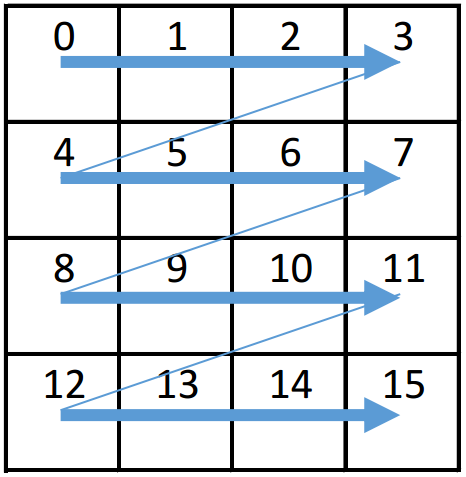
\includegraphics[width=\linewidth]{images/parcours_rowscan.png}
		\caption{\textbf{rowscan} : parcours horizontal du plateau}\label{fig:parcours_rowscan}
		\endminipage\hfill
		\minipage{0.32\textwidth}
		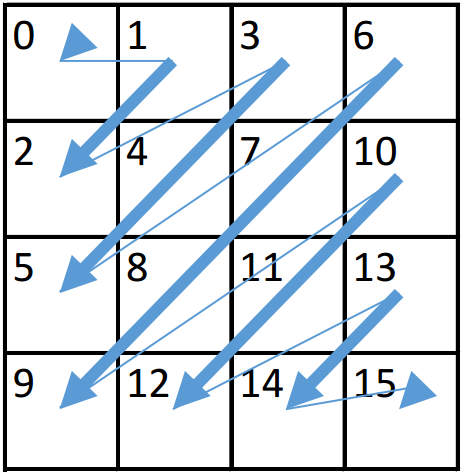
\includegraphics[width=\linewidth]{images/parcours_diagonal.png}
		\caption{\textbf{diagonal} : parcours diagonal du plateau}\label{fig:parcours_diagonal}
		\endminipage\hfill
		\minipage{0.32\textwidth}
		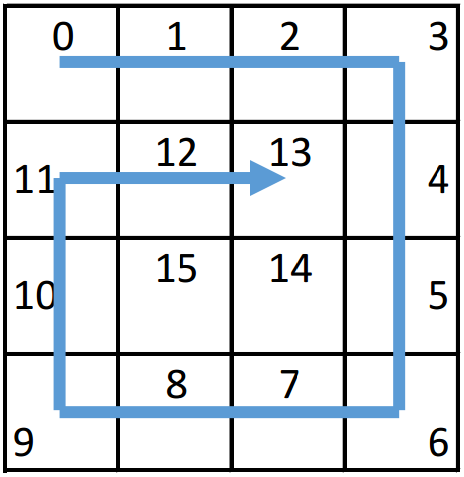
\includegraphics[width=\linewidth]{images/parcours_spiral-in.png}
		\caption{\textbf{spiral-in} : parcours en spirale fermente du plateau}\label{fig:parcours_spiral-in}
		\endminipage\hfill
	\end{figure}
	\begin{figure}[H]
		\minipage{0.32\textwidth}
		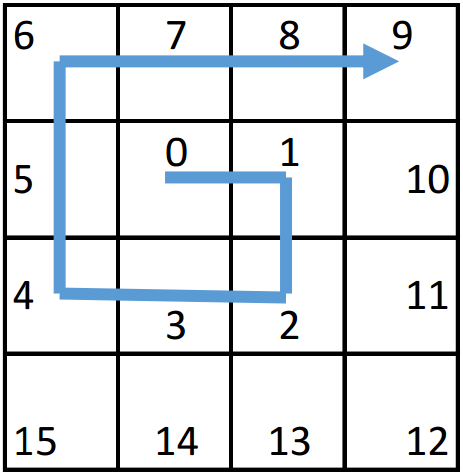
\includegraphics[width=\linewidth]{images/parcours_spiral-out.png}
		\caption{\textbf{diagonal} : parcours en spirale ouvrante du plateau}\label{fig:parcours_spiral-out}
		\endminipage\hfill
		\minipage{0.32\textwidth}
		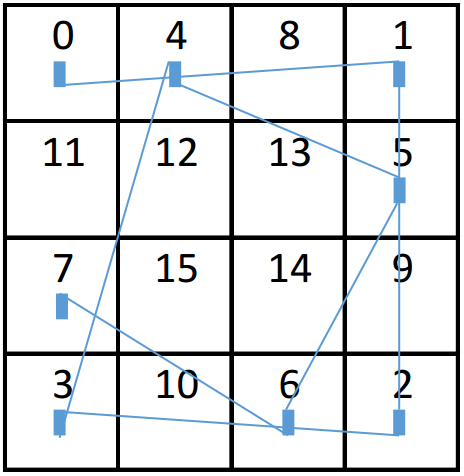
\includegraphics[width=\linewidth]{images/parcours_quad-spiral-in.png}
		\caption{\textbf{quad spiral out} : parcours avec quatre spirales fermentes}\label{fig:quad-spiral-in}
		\endminipage\hfill
		\minipage{0.32\textwidth}
		\ %don't touch this !
		\endminipage\hfill
	\end{figure}
	
	Le choix des pièces (valeurs) est fait dans l'ordre lexicographique.
	
	Les données utilisés pour l'étalonnage sont les suivants :
	
	\begin{description}
		\item[Première solution] : le temps et la quantité de n\oe uds nécessaires pour trouver la première solution (chaque instance peux en avoir plusieurs)
		\item[Nombre total de solutions] : pour estimer les placement des solutions dans l'arbre
		\item[Nombre total de n\oe uds] : pour pouvoir estimer la rapidité de l'algorithme pour trouver la première solution
		\item[Temps total] : pour connaître si l'algorithme utilisé est plus performant que celui d'avant
	\end{description}
	
	--- [résumé]
	
	Afin de pouvoir partir sur de bonnes bases, plusieurs différents méthodes de parcours (quel chemin prendre pour résoudre mon plateau) ont été utilisé, afin de voir quel parcours est le plus performant pour la résolution brute. En sachant que le nombre de noeuds/sec est la même, l'unité de mesure est le nombre de noeuds.

	Les différents types de parcours sont :

	\begin{description}
		\item[rowscan]: on pose les pieces en lignes horizontales sur le plateau
		\item[diagonal]: on pose les pieces en diagonal
		\item[spiral in]: on dispose les pièces en spirale en partant de l'exterieur
		\item[spiral out]: idem que spiral in mais en partant de l'intérieur vers l'extérieur
	\end{description}

	Ces différents types de parcours ont été testés sur plusieurs instances de taille variable.

	\subsection{Smartforce}

	La smartforce repose sur la quantité de données qu'elle possède. Par conséquent, il est important que ces données soient bien organisés, afin de pouvoir les traiter avec aise. Ces données sont organisés pour former des modèles. Chaque modèle peut être interprété comme un point de vue différent par rapport au problème.
	
	On note aussi l'introduction de nouvelles méthodes de parcours :
	
	\begin{itemize}
		\item Choix de variable :
		\begin{itemize}
			\item\textbf{Optimiste} : on choisit la variable qui à le plus grand domaine
			\item\textbf{Pessimiste} : on choisit la variable qui à le plus petit domaine
		\end{itemize}
		\item Choix de valeur :
		\begin{itemize}
			\item \textbf{Lexicographique} : utilisé par défaut par la bruteforce, on choisit la valeur suivante dans l'ordre par défaut.
			\item \textbf{Optimiste} : la valeur dont le domaine est le plus grand
			\item \textbf{Pessimiste} : la valeur dont le domaine est le plus petit
		\end{itemize}
	\end{itemize}
	
	Différents modèles seront donc présentés par ordre de difficulté, car, afin de fournir des types de données variés, il est nécessaire d'abstraire le problème initial.
	
--- [résumé]

	Une fois la valeur étalon fixée, il est maintenant facile de mettre en place un autre approche du problème qui à pour principe de cumuler une grande quantité de donnée pour faire face au nombre exponentiel de possibilités.

	Les différents types de données (nommés modèles) sont comme différents points de vues du problème. Ils sont plus ou moins utiles, mais la force réside dans leur union. Mais surtout, ils permettent de mettre en place le concept d'ouvertures et finales.

	\subsubsection{CaPi}

	CaPi est le plus simple modèle représentant le problème. Il à pour variable les cases (identifiés par un numéro ou par ses coordonnées sur le plateau) et pour valeur les pièces (identifiés par un numéro et par leurs rotation). C'est aussi lui qui est utilisé comme modèle par défaut pour le choix des valeurs et variables.
	
	En somme, chaque pièce est associé aux cases sur laquelle elle peut être posée et inversement, chaque case contient la liste des pièces qu'elle peux avoir.
	
	\begin{rem}
		Le domaine des cases est un peu plus complexe : une pièce donnée peux être placée sur la case \enquote{jusqu'à 4 fois} (à plusieurs rotation différentes). Par conséquent, lorsque l'on met à jour le domaine de la case (en posant la pièce sur une autre case), on supprime toutes les occurrences de cette pièce du domaine en question.
		
		Par conséquent, chaque pièce possède en vérité quatre domaines distincts (correspondant à chaque rotation de la pièce).
	\end{rem}

--- [résumé]
	L'approche CaPi (abbréviation de Cases/pieces) est l'approche la plus naive, elle permet de définir quelle piece peut être placée sur telle case et inversement, quelle case peux avoir telle piece.

	Cette approche est l'interaction la plus basique de notre problème. C'est aussi celle-ci qui est utilisée en bruteforce.

	\subsubsection{BoCo}
	
	Le modèle BoCo (Bordures/Couleurs) est une approche bien plus fine, elle découle de l'abstraction de CaPi.
	
	Si l'on connait le domaine d'une case. On connaît les pièces qui peuvent être posés dessus. Par conséquent, on définit une \textbf{Bordure} comme une sous-partie d'une case.
	
	\begin{exmp}
		Prenons la case 0, en 0,0 sur le plateau. Elle peux contenir 4 pièces (\no 0,1,2,3 ; ce sont toutes des pièces de coin) à la rotation 0.
		
		
		\minipage[t]{0.29\textwidth}
		Si l'on décompose la case, celle-ci contient 4 faces :
		
		\begin{figure}[H]
			\includestandalone[width=\linewidth]{graphics/case}

			\caption{Détails d'une case}\label{fig:case}
		\end{figure}
		
		Les bords 1 et 2 étant gris, il n'est pas nécessaire de les représenter. 
		\endminipage\hfill
		\minipage[t]{0.29\textwidth}
	
		On décompose ensuite les 4 pièces :
		\begin{figure}[H]
			\includestandalone[width=\linewidth]{graphics/4_pieces}
			
			\caption{Couleurs des 4 pièces}\label{fig:4_pieces}
		\end{figure}
		\endminipage\hfill
		\minipage[t]{0.29\textwidth}
			On associe ensuite les couleurs et leur occurence à chaque bord :
			\begin{figure}[H]
				\includestandalone[width=\linewidth]{graphics/4_pieces_on_bordure}
				
				\caption{Occurrences et couleurs de bordures}\label{fig:4_pieces_on_bordure}
			\end{figure}
		\endminipage\hfill
		
	---	[en cours]
	\end{exmp}
	
	--- [résumé]

	L'approche BoCo (Bordure/Couleur) est bien plus fine : si l'on connait quelle piece est sur telle case, on sait quelle couleur peux se placer sur telle bordure [de la case]. Elle permet d'implémenter un système de mis à jour bien plus performant car ne nombre de couleurs est bien plus petit que le nombre de pièces.

	\begin{exmp}
		Si une couleur disparait, alors tt les pièces ayant cette couleur ne peuvent plus être placés à cette case, par conséquent, les autres bords de la case ont (probablement) des couleurs qui disparaissent aussi (propagation de la disparition).
	\end{exmp}

	\subsubsection{Corolles}

	Grace aux visions CaPi et BoCo, il est possible de pré-calculer des zones du plateau nommés corolles, ceux-ci contiennent tous les cas possibles dans cette zone donnée.

	Le nombre de cas possible étant très important, il est nécessaire de le classer. Les corolles peuvent êtres identifiés grâce à plusieurs critères.

	\begin{itemize}
		\item taille du plateau
		\item l'orientation de la corolle
		\item La pièce (et sa rotation) à l'origine de la corolle
		\item La case à l'origine de la corolle
		\item La taille de la corolle
	\end{itemize}

	\paragraph{position et orientation des corolles}

	\subsubsection{BoCoDiag}

	\newpage
	\section{Manuel d'utilisation}

Dans cette partie nous verrons comment utiliser les différents outils développés pendant la durée du stage.

	\subsection{Pré-requis}
	
	Afin de pouvoir manipuler avec aise l'ensemble des outils présentés ici, il est vivement conseillé de connaître le fonctionnement global d'un Git \autocite{git}.
	
	L'ensemble des outils présentés ici sont hébergés sur un dépot privé de l'UM \autocite{gitlab:eternity}.

	\subsection{EternityII}
	
	\textbf{Pré-requis} : Afin de pouvoir utiliser ce logiciel il est nécessaire de pouvoir compiler du code C++11 et utiliser la commande \enquote{\lstinline[columns=fixed,language=bash]{make}}.
	
	Le programme \textbf{EternityII} est le programme principal développé le long de l'année et du stage. Le code source peux être récupéré ici : \url{https://gitlab.info-ufr.univ-montp2.fr/EternityII/EternityII} (dépôt privé).
	
	Le dépot contient deux versions du programme :
	
	\begin{itemize}
		\item La version basique pour la résolution bruteforce
		\item la résolution smartforce
	\end{itemize}

	\subsubsection{Bruteforce}
	
	La version bruteforce se trouve sur la branche v0.2.2-bruteforce \autocite{gitlab:eternity_bruteforce}. L'interaction avec l'application se fait dans le main :
	
	\begin{lstlisting}[language=c++, caption={Parcours bruteforce sur plusieurs tailles du plateau, en affichant tous les résultats des différents parcours}]
int main()
{
    for (int i = 4; i < 8; ++i) {
        ostringstream str;
         // nom du fichier d'entree contenant l'instance
        str << "assets/pieces_" << i << "x" << i << ".txt";
        FileIn file_in(str.str().c_str());
        Jeu jeu = file_in.initJeu(); // initialise le jeu
        // initialise la classe chargee de la resolution
        Generator generator(jeu); 
        // Affiche les resultats pour tous les parcours
        generator.multipleGeneration(); 
    }
}
	\end{lstlisting}
	
	Pour effectuer un parcours spécifique, la dernière ligne doit être changée :
	
	\begin{lstlisting}[language=c++, caption={Parcours bruteforce sur plusieurs tailles du plateau, en affichant tous les résultats du rowscan}]
int main()
{
    for (int i = 4; i < 8; ++i) {
        ostringstream str;
        // nom du fichier d'entree contenant l'instance
        str << "assets/pieces_" << i << "x" << i << ".txt"; 
        FileIn file_in(str.str().c_str());
        Jeu jeu = file_in.initJeu(); // initialise le jeu
        // initialise la classe chargee de la resolution
        Generator generator(jeu); 
        // Affiche les resultats du parcours
        generator.parcoursBruteForce(Generator::PARCOURS_ROW,0); 
    }
}
	\end{lstlisting}
    
	Les différentes constantes pour le parcours sont :
    
	\begin{itemize}
		\item \lstinline[language=c++]|Generator::PARCOURS_ROW|
		\item \lstinline[language=c++]|Generator::PARCOURS_DIAGONAL|
		\item \lstinline[language=c++]|Generator::PARCOURS_SPIRALE_IN|
		\item \lstinline[language=c++]|Generator::PARCOURS_SPIRALE_OUT|
	\end{itemize}
	
	Les fichiers d'instances se trouvent dans le dossier \enquote{assets}.
	
	Le résultat est affiché en Markdown \autocite{markdown}.
	
	\subsubsection{Smartforce}
	
	La résolution smartforce est en cours de développement, malgré le fait que le framework (outil de développement) soit fini. L'implémentation de CaPi est incomplète et renvoie des données non cohérentes.
	
	Le fonctionnement du framework est explicité dans le manuel technique.
	
	\subsection{EternityII--corolle\_generator} 
	
	Le code de ce programme peux être trouvé ici : \url{https://gitlab.info-ufr.univ-montp2.fr/EternityII/EternityII-corolle_generator} (dépôt privé).
	
	Le code source est inspiré du programme de bruteforce.
	
	\textbf{Utilisation}
	
	Compiler le programme en utilisant make (linux).
	
	Le programme accepte deux arguments :
	
	\begin{itemize}
		\item Le fichier d'instance (qui peux être trouvé dans le dossier assets)
		\item Le hamming maximal à générer (2 par défaut).
	\end{itemize}
	
	\begin{exmp}
		La commande \lstinline[language=bash]|$ ./main pieces_10x10.txt 2|
		
		Génèrera les corolles de toutes les zones en hamming 1 et 2 pour un 10.
	\end{exmp}
	
	\textbf{Personnalisation}
	
	Il est malgré tout possible de forcer le programme à ne générer qu'une zone et un hamming spécifique.
	
	En modifiant les lignes (10-14) du fichier main.cpp :
	
	\lstinputlisting[language=c++, firstline=9]{code/corolle.cpp}
	
	en 
	
	\begin{lstlisting}[language=c++]
generator.initGeneration(0,0,1) // x,y,hamming
	\end{lstlisting}
	
	\subsection{EternityII--cardinality\_counter} 
	
	Le code de ce programme peux être trouvé ici : \url{https://gitlab.info-ufr.univ-montp2.fr/EternityII/EternityII-cardinality_counter} (dépôt privé).
	
	Ce programme est en python, il compte le nombre de pièces uniques à chaque position dans la corolle. Il prends deux arguments :
	
	\begin{itemize}
		\item Le fichier corolle.
		\item (optionnel) \enquote{--o} sauvegarde le résultat dans un fichier du même nom avec \enquote{stat\_} préfixé
	\end{itemize}
	
	\begin{exmp}
		\lstinline[language=bash]|$ python main.py corolle.txt -o|
		Traite le ficher et sauvegarde les comptes dans un fichier nommé \lstinline|stat_corolle.txt|
	\end{exmp}
	
	\subsection{EternityII--corolle\_rotator}
	
	Le code de ce programme peux être trouvé ici : \url{https://gitlab.info-ufr.univ-montp2.fr/EternityII/EternityII-corolle_rotator} (dépôt privé).
	
	\textbf{Description}
	
	Génère un fichier de la corolle à la rotation voulue, en fonction du fichier initial.
	
	\textbf{Usage}
	
	\lstinline[language=bash]|$ python main.py file_path [-o output_file, -r rotation]|
	
	\begin{itemize}
		\item \lstinline|file_path| est le chemin vers le fichier de corolle
		\item \lstinline|-o| ou \lstinline|--output| est le chemin vers le fichier généré
		\item \lstinline|-r| ou \lstinline|--rotation| est la rotation souhaitée (entre 0 et 3)
	\end{itemize}
	
	\begin{rem}
		si \lstinline|-o| est spécifié, alors \lstinline|-r| doit l'être aussi.
	\end{rem}
	\begin{rem}
		si \lstinline|-r| n'est pas spécifié, alors il générera les 3 rotation complémentaire au fichier
	\end{rem}
	
	Le fichier de sortie est généré dans le même répertoire que le fichier d'entrée.
	
	\newpage
	\section{Manuel Technique}

Dans cette partie, sera expliqué le fonctionnement de chaque application, en particulier, le framework développé pour la smartforce.

Le but est de fournir assez d'information afin de faciliter le maintient et la manipulation des applications développées.

	\subsection{EternityII (bruteforce)}
	
Cette application a été bâtie de façon à pouvoir rapidement intégrer de nouvelles méthodes de parcours. Elle intègre aussi différents outils de manipulation de fichiers.

Son fonctionnement est simple. Chaque classe accomplit une certaine tâche spécifique \autocite{wiki:kissprinciple}.

D'abord, on charge le fichier d'instance (main.cpp) grâce à la classe \lstinline[language=c++]|FileIn|. 

Une fois les données récupérés du fichier, le \lstinline[language=c++]|Jeu| est initialisé (les différentes \lstinline[language=c++]|Pieces| ainsi que le plateau).

Le jeu est ensuite envoyé à \lstinline[language=c++]|Generator| qui va initialiser les données nécessaires à la résolution. 

Grâce à la fonction  \lstinline[language=c++]|Genetrator::multipleGeneration| ou directement  \lstinline[language=c++]|G::parcoursBruteforce|, on définit le type de parcours. En fonction du type de parcours, le chemin est initialisé par  \lstinline[language=c++]|G::coordinatesCreator|. 

Une fois le chemin sur le plateau initialisé (voir \autoref{fig:parcours_rowscan}), le solveur (\lstinline[language=c++]|G::generationRecursive|) est lancé . Celui-ci va, en fonction des coordonnées, tester si les pièces peuvent être placés (les pièces de coins ne seront testés que sur les coins, \dots). 

Lorsqu'une solution est trouvée, l'évenement \lstinline[language=c++]|G::solutionFoundEvent| est déclenché. 

	\subsection{EternityII--corolle\_generator}
	
Le générateur de corolle est directement inspiré de l'application de bruteforce. Au lieu de résoudre tout le plateau, il résout une sous-partie de celui-ci (une corolle).

Lorsqu'une corolle est trouvée, au lieu de déclencher l'évènement, il va copier les pièces dans un objet \lstinline[language=c++]|Corolle|, la frontière de la corolles est aussi déterminée à ce stade. La corolle et la frontière sont envoyés à la fonction \lstinline[language=c++]|Generator::writeInFile|.

Si un fichier est déjà ouvert, celle-ci vérifie si ces données sont identiques:

\begin{itemize}
	\item si la taille du plateau est identique
	\item le hamming de la corolle
	\item la pièce centrale (et son orientation) 
	\item la zone de la corolle (représentée sous forme de coordonnées $(x,y)$)
\end{itemize}
	
	Si aucun fichier n'est ouvert ou que l'une de ces données est différente, un nouvel objet \lstinline[language=c++]|FileOut| est créé et remplace le précédent.
	
	\lstinline[language=c++]|FileOut| va alors créer ou ouvrir (en supprimant le contenu) le fichier et écrire 4 lignes contenant toutes les informations de la corolle. 
	
	Les deux premières lignes sont sous cette forme :
	
	\begin{exmp}\ 
		
		\begin{lstlisting}[language=bash]
# taille rotation_corolle no_piece rotation x y hamming nb_pieces
# 6 0 0 0 0 0 1 3
	\end{lstlisting}
	\end{exmp}
	
	Sera ensuite écrit la ligne contenant les information de la corolle :
	
	\begin{exmp}
		\lstinline[language=bash]{0:0;5:1;6:0;;|3;4;5;6;7;;;;;;;0}
	\end{exmp}
	
	Si les données du fichier sont identiques, alors la corolle est ajoutée au fichier grâce à la fonction \lstinline[language=c++]{FileOut::put}.
	
	\subsection{EternityII--cardinality\_counter} 
	
On parcours d'abord le fichier contenant les corolles (\lstinline[language=python]|count()|) comptant le nombre de pièces uniques à chaque position (\lstinline[language=python]|count_pieces()|).

Vient ensuite \lstinline[language=python]|put_on_plate()| qui se charge de convertir chaque position en coordonnées $(x,y)$ et en y mettant le nombre d'occurences.

Enfin \lstinline[language=python]|display_plate()| qui affiche ou enregistre, en fonction des options, le plateau avec les occurences.

	\subsection{EternityII--corolle\_rotator}
	
Lorsqu'une corolle est tournée, non seulement les pièces sont tournées, mais l'ordre de parcours change aussi (voir \autoref{fig:corolle_zone_orientee} et \autoref{fig:corolle}). Par conséquent, il suffit non seulement de tourner les pièces \lstinline[language=python]|pieces_rotate()| mais aussi de \enquote{shifter} les pièces.

\begin{exmp}
	Prenons une corolle en $(1,1)$ (Z5 dans la \autoref{fig:corolle_zones_h_1}).
	on obtient donc : \\
	\begin{minipage}{0.24\textwidth}
		\begin{figure}[H]
			\centering
			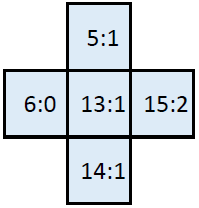
\includegraphics[width=\linewidth]{images/corolle_ex_orientee}
			\caption{Exemple de corolle de hamming 1 en $(1,1)$}
			\label{fig:corolle_ex_orientee}
		\end{figure}
	\end{minipage}\hfill
	\begin{minipage}{0.24\textwidth}
		\begin{figure}[H]
			\centering
			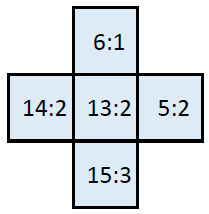
\includegraphics[width=\linewidth]{images/corolle_ex_orientee_1}
			\caption{Exemple de corolle de hamming 1 en $(5,1)$ }
			\label{fig:corolle_ex_orientee_1}
		\end{figure}
	\end{minipage}\hfill
	\begin{minipage}{0.24\textwidth}
		\begin{figure}[H]
			\centering
			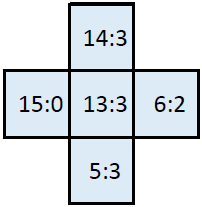
\includegraphics[width=\linewidth]{images/corolle_ex_orientee_2}
			\caption{Exemple de corolle de hamming 1 en $(5,5)$}
			\label{fig:corolle_ex_orientee_2}
		\end{figure}
	\end{minipage}\hfill
	\begin{minipage}{0.24\textwidth}
		\begin{figure}[H]
			\centering
			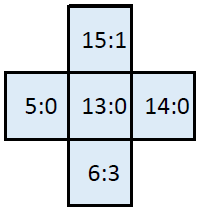
\includegraphics[width=\linewidth]{images/corolle_ex_orientee_3}
			\caption{Exemple de corolle de hamming 1 en $(1,5)$}
			\label{fig:corolle_ex_orientee_3}
		\end{figure}
	\end{minipage}\hfill
		
		
	Sous forme de texte, en excluant la frontière on à donc :
	\begin{lstlisting}
13:1;15:2;14:1; 6:0; 5:1|...
13:1; 5:2;15:3;14:2; 6:1|...
13:1; 6:2; 5:3;15:0;14:3|...
13:1;14:0; 6:3; 5:0;15:1|...
	\end{lstlisting}
	
	On remarque que les 4 dernières pièces (appartenant au hamming 1) bouclent en se décalent de 1 à chaque fois (d'où le fait de \enquote{shifter} les cases).
\end{exmp}

Ce comportement marche sur tous les Hammings. Les pièces appartenant au hamming 2 de la corolle \enquote{shiftent} de 2, et ainsi de suite.

Cette action est gérée par \lstinline[language=python]|pieces_shift|  pour les pièces et \lstinline[language=python]|color_shift| pour la frontière.


\subsection{EternityII(smartforce)}

Le code source se trouve sur : \url{https://gitlab.info-ufr.univ-montp2.fr/EternityII/EternityII/commits/feature/framework_refactoring}

Cette application est composée de deux parties :

\begin{itemize}
	\item le core de l'application (le framework)
	\item l'app qui contient les différentes données nécessaires à la résolution
\end{itemize}

Cette application à été mise en place pour plusieurs raisons :
\begin{itemize}
	\item Pouvoir organiser un grand nombre de données
	\item interconnecter les données entre eux pour optimiser la mise à jour des informations
	\item fournir une platforme modulaire afin de pouvoir facilement intégrer de nouvelles données
	\item mettre en place des systèmes de résolutions alternatifs
	\item implémenter facilement et rapidement de nouvelles façon de parcourir l'arbre
\end{itemize}

\subsubsection{Principe}

Avant d'aborder l'implémentation, il est important de comprendre le principe de l'application.

Le framework est décomposé en 4 parties distinctes :

\begin{enumerate}
	\item Les Modèles
	\item Les Contraintes
	\item Le \enquote{PathFinder}
	\item Le Solveur
\end{enumerate}


\paragraph{Les contraintes}

Les modèles sont contraints par les contraintes, ceux-ci sont chargés de la propagation des données entre les modèles.

\paragraph{Les modèles}

Un modèle est un objet chargé de la manipulation d'une donnée lors de la résolution du problème. Il avertit les modèles auquel il est connecté lors d'un changement utile dans ses données via les contraintes.

\paragraph{Le Pathfinder}

Le PathFinder est connecté à des modèles de référence. Grâce à eux, il détermine le choix de valeur et le choix de variable.

\paragraph{Le solveur}

Le solveur progresse dans l'arbre, à chaque n\oe ud il récupère grâce au PathFinder le n\oe ud suivant à atteindre. Il envoie ensuite la décision aux modèles de références. Si le Pathfinder n'en trouve pas, il envoie alors un ordre de rollback vers le n\oe ud précédent.
\newpage

\subsubsection{Fonctionnement}

\paragraph{Solveur et PathFinder}

Le \textbf{solveur} à un rôle simple, c'est celui qui donne l'ordre de continuer ou non, c'est aussi celui qui est chargé de parcourir l'arbre des possibilités.
Il utilise les ordres suivants :

\begin{description}
	\item [resolve] qui lance la résolution du problème
	\item [resolve(profondeur)] qui détermine le choix de variable (utilise le pathfinder)
	\item [resolve(variable, profondeur)] teste récursivement toutes les valeurs et rappelle \lstinline[language=c++]|resolve(profondeur+1)|. \`{A} la fin de résolution des noeuds fils, un rollback partiel est effectué (on dénie le n\oe ud fils qui vient de se terminer).
	Une fois que toutes les valeurs ont été testés pour la variable actuelle, on fait un rollback total pour revenir au n\oe uds parent (qui déniera le n\oe uds actuel comme choix de variable).
\end{description}

Il contient deux modèles qui sont les points d'entrée vers les autres modèles. C'est à ces deux modèles que les données relatives aux choix de variable et de valeur vont être envoyées.

\begin{figure}[H]
\centering
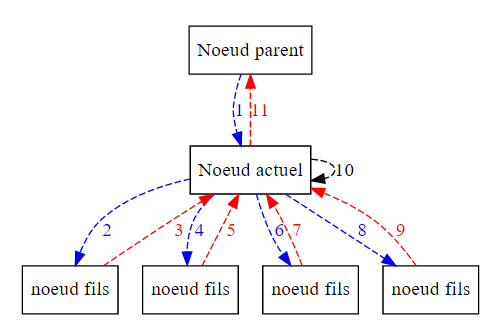
\includegraphics[width=\linewidth]{images/parcours_noeuds}
\caption[Fonctionnement d'un solveur]{Fonctionnement d'un solveur.\\	
	 En bleu, la progression d'un noeud à l'autre.\\ En rouge, un rollback partiel. \\ En noir, un rollback total.\\}
\label{fig:parcoursnoeuds}
\end{figure}

Le \textbf{pathfinder} aide le solveur à prendre des décisions. Il est associés à classes, l'un pour le choix de variable (ex: cases en rowscan), l'autre pour le choix de valeur (ex: pièces en lexico). Il contient 4 ordres :
\begin{description}
	\item [hasNextVariable] qui renvoi vrai s'il existe une variable à une profondeur donnée.
	\item [nextVariable] qui renvoi une variable suivant la stratégie de variable utilisée.
	\item[hasNextValue] renvoi vrai s'il existe une valeur à la variable et la profondeur actuelle
	\item[nextValue] renvoi une valeur suivant la stratégie de utilisée.
\end{description}

Il est important de noter que le pathfinder et le solveur doivent utiliser les mêmes données pour les valeurs et variables, lorsque ceux-ci sont envoyés aux modèles.

\begin{exmp}
	Afin d'éviter, par exemple, d'envoyer les identifiants de BoCo à un solveur CaPi.
\end{exmp}

\subsubsection{Modèles et contraintes}

Les modèles sont interconnectés entre eux grâce aux contraintes.

\begin{figure}[H]
	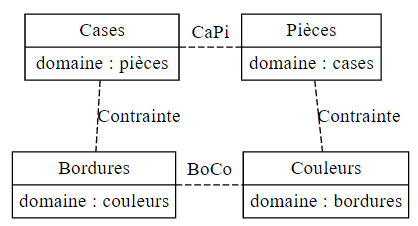
\includegraphics[width=\linewidth]{images/modeles_contraintes}
	\caption{Structure des modèles et des contraintes pour EternityII}
	\label{fig:modeles_contraintes}
\end{figure}

Chaque modèle doit pouvoir effectuer ces actions :

\begin{description}
	\item[allow] autorise un couple de données (ex : CaPi) en tant que variable et valeur pour le n\oe ud actuel. Cela déclenche 2 actions : 
	\begin{itemize}
		\item dénie toutes les autres valeurs pour la variable et réciproquement.
		\item propage l'autorisation du couple aux autres modèles.
	\end{itemize}
	\item[denyOne] dénie le couple de valeur/variable pour la donnée actuelle. on peux aussi dénier définitivement un couple (utile lors d'un parcours en largeur de l'arbre).
	\item[addOne] Utilisé lors de l'initialisation, il permet d'ajouter des données
	\item[rollback(profondeur, total/partiel)] permet de rétablir le modèle à une profondeur antérieure partiellement ou totalement.
\end{description}
\newpage

\subsubsection{Fonctionnement global}

L'ensemble des éléments est gérée par la classe EternityII, elle est aussi chargée de l'hébergement de tous les autres objets.

\begin{figure}[H]
\centering
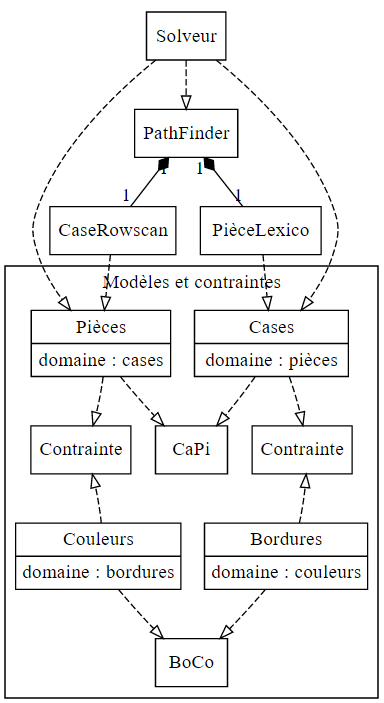
\includegraphics{images/model_simplifie}
\caption{Modèle simplifié du fonctionnement du framework}
\label{fig:model_simplifie}
\end{figure}

Le solveur demande et envoie le couple CaPi depuis le pathfinder aux modèles d'entrées (CaPi), ceux-ci sont chargés de propager l'information aux autres modèles via les contraintes.

\subsubsection{Conseils pour le développement de l'application}

Tout solveur doit hériter de core/SolverInterface.h

Tout choix de variable doit implémenter VariableInterface

Tout choix de valeur doit implémenter ValueInterface

Toute contrainte doit implémenter ConstraintInterface

Tout modèle doit implémenter ModelInterface

Toute donnée transmise d'une classe à l'autre doit implémenter DataInterface

La création de toutes les classes ont lieu dans \lstinline[language=c++]|EternityII::bootstrap|

Tous les fichiers liées à l'application doivent se trouver dans le dossier app/.

Certains commentaires sont à lire lors de toute modification, ils sont préfixés par différents mots-clés :

\begin{description}
	\item[unused :] la fonction n'est pas utilisée
	\item[entrypoint :] lire le commentaire si le point d'entrée à changé
	\item[minimal importance :] La tache à faire n'est pas indispensable au fonctionnement de l'application
	\item[advice :] indique la marche à suivre
	\item[dangerous :] la fonction ou l'algorithme est fragile (dangereuse à utiliser ou a modifier).
\end{description}

	\newpage
	\section{Resultats}

Dans cette partie, nous verrons les résultats et déductions qui ont été faites à partir des différentes approches. Elle évoquera aussi ce qui à été accompli et ce qui reste à faire.

Les résultats et déductions seront cités par ordre chronologique, il est donc normal que certaines approches soient invalidés.

L'implémentation et le fonctionnement interne des application sont explicités dans le manuel technique, malgré tout, certaines implémentations seront expliquées ici pour justifier les décisions prises durant le stage.

De plus, grâce au développement en parallèle d'un solveur en programmation par contraintes \autocite{choco} par Mr Bourreau nous apporte un certain recul sur les données reçus.

	\subsection{Bruteforce}
	
	Les résultats de la bruteforce suivent ce qui avait été prédit. Malgré un certain niveau d'optimisation du programme, la plus grande instance résolue est de taille 6.
	
	Le puzzle de taille 7 n'as pas pu être parcouru en 9 heures de calcul. Malgré tout, la première solution de l'instance se trouvait au n\oe ud 10548049 et à été trouvée en 31.7344 secondes en rowscan.
	
	D'après les résultats le choix de variable le plus performant est le \enquote{rowscan} [\autoref{annexe:bruteforce}]. On remarque aussi que le nombre de n\oe uds total et le temps écoulé augmente de façon exponentielle en fonction de la taille de l'instance.
	
	\begin{note}
		La programmation par contrainte à l'air d'être plus performante que le parcours naïf en bruteforce d'après la \autoref{fig:results_bruteforce_graphique_compare}.
	\end{note}
	
	\subsection{Smartforce}
	
	Les valeurs étalons pour les choix de variables dynamiques (optimiste/pessimiste) qui ont été implémentés sur un modèle \textbf{CaPi}, elles se sont avérées moins performantes qu'un parcours basique.
	
	La raison est simple : il est possible de recréer le même cas en parcourant de différentes façons. Par conséquent, le nombre de n\oe uds augmente sans pour autant parcourir de nouvelles possibilités.
	
	\begin{exmp}
		Soit un plateau composé de deux cases et par conséquent, de deux pièces. Si je pose d'abord ma pièce sur la première case, puis sur la deuxième. Le résultat sera le même que si je pose d'abord l'autre pièce sur la deuxième case puis que je fasse la première.
		
		Donc, j'ai deux façons de trouver le même résultat.
	\end{exmp}
	
	Le choix de valeur dynamique, décident du chemin à chaque n\oe uds, il fait plusieurs fois la même combinaison, mais avec un chemin différent.
	
	Les tests effectués sur les choix de valeur dynamiques ont obtenus les mêmes résultats que pour le \textbf{rowscan} car aucune mise à jour par propagation n'a pas été implémentée pour CaPi (non performant).
	
	Le modèle \textbf{BoCo} est en cours d'implémentation, mais ne fournit pas des résultats pertinent. Le problème se trouve dans le mécanisme de mise à jour par propagation.
	
	\subsection{Corolles}
	
	Afin de pouvoir assimiler le fonctionnement des corolles dans la pratique, il est important de tenir compte de la quantité volumineuse d'information que génère ce modèle (voir \autoref{annexe:smartforce}).
	
	A titre d'exemple, le nombre de corolles en hamming 2 pour une instance de taille 6 (non rotationnées) est de 850694772. Avec un stockage non optimisé des corolles, l'espace occupé par ces corolles s'élève à environ 90GB.
	Par extension, on peux en déduire que pour une instance de taille 7, l'espace occupé par l'ensemble des corolles avoisinera au moins 1TB (en prenant la valeur de la \autoref{table:count_hamming_2} comme valeur max, et en supposant que l'espace occupé par une corolle est la même).
	
	Ce stockage avait un défaut important, il n'était pas optimisé pour le stockage mais pour pouvoir manipuler avec aise les corolles.
	
	Une corolle etait stockée de cette manière : chaque pièce était identifiée par un numéro et sa rotation, l'ensemble des pièces était séparés par un charactère (;) et disposés dans un ordre spécifique (voir \autoref{fig:corolle}). Suivait ensuite la frontière, composée de couleurs qui étaient aussi séparés par un charactère (;). Évidemment, si la corolle etait réduite, les cases et frontières manquantes étaient remplacées par un vide.
	\begin{exmp}
		\lstinline[columns=fixed]{0:0;5:1;6:0;;|3;4;5;6;7;;;;;;;0}
	\end{exmp}
	
	Une corolle étant une sous-partie du plateau, un ensemble de corolles peux être représenté sous forme d'arbre. Lors de la création de la corolle, on parcours tout simplement l'arbre en profondeur. Ainsi, dans le fichier, deux lignes adjacentes se ressemblent fortement.
		\begin{figure}[H]
			\centering
			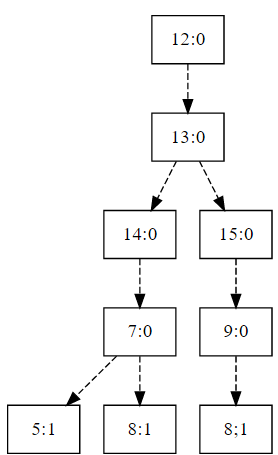
\includegraphics[width=0.3\linewidth]{images/corolle_tree}
			\caption{Représentation sous forme d'arbre d'un exemple de corolles possibles}
			\label{fig:corolle_tree}
		\end{figure}
	
	
	\begin{exmp}\ 
		
		\begin{lstlisting}
0:0;5:1;6:0;;|3;4;5;6;0;;;;;;;0
0:0;5:1;7:0;;|3;4;5;3;0;;;;;;;0
		\end{lstlisting}
		
	\end{exmp}
	
	On peux donc optimiser en spécifiant à partir quelle pièce se fait l'optimisation.
	
	Nous obtenons donc :
	
	\begin{exmp}
		\ 
		
		\begin{lstlisting}
0>0:0;5:1;6:0;;|3;4;5;6;0;;;;;;;0
1>7:0;;|3;4;5;3;0;;;;;;;0
		\end{lstlisting}
	\end{exmp}
	
	Grâce à ce procédé, le fichier de 90GB est passé à 20GB, ce qui nous donne une optimisation de $70\%$ environ. Ceci étant, il est intéressant de noter que la compression de ces fichier grâce à LZMA \autocite{wiki:lzma} permet de réduire de $98\%$ le volume du fichier. Mais la compression exige un certain délai afin de pouvoir exploiter les fichiers compréssés, ce qui limite son utilisation.
	
	Il existe une dernière approche, qui se base sur un constant simple :
	dans une corolle de hamming 1, les pièces adjacentes à la pièce centrale sont indépendantes les uns des autres. Il suffit donc de lister à chaque position les pièces qui peuvent y être posés, puis lorsqu'il y a nécessité de créer une corolle, parcourir les positions en fixant une pièce. Toutes les corolles sont possibles, tant que le chemin ne possède pas deux fois la même pièce.
	
	\begin{exmp}
		Reprenons l'exemple précédent en y rajoutant une ligne:
		
		nous avons donc
		\begin{tabular}{|c|c c c|}
			\hline 
			Positions & 0 & 1 & 2 \\ 
			\hline 
			 & $0:0$ & $5:1$ & $6:0$ \\
			  & $0:0$ & $5:1$ & $7:0$ \\
 & $0:0$ & $6:1$& $7:0$ \\
 \hline
		\end{tabular}
		
		il suffit donc d'enregistrer dans le fichier :
		
		\begin{lstlisting}
			0:0;5:1;6:0
			   ;6:1;7:0
		\end{lstlisting}
		
		Tant que l'on ne prend pas \lstinline[columns=fixed]{0:0;6:1;6:0} tous les autres cas sont possibles.
	\end{exmp}
	
	Plus théoriquement, on fait un produit cartésien entre les ensembles de chaque position et l'on en obtient une corolle.
	
	Le soucis, c'est que cette méthode fonctionne en hamming 1 car les pièces de H1 sont indépendantes de les unes des autres. En H2, l'approche est plus complexe : les pièces de H2 sont dépendants des pièces de H1. Or, on vient de déterminer un moyen de stocker les corolles. Il suffit de spécifier quel chemin emprunter en H1 (l'identifier) puis d'appliquer la même méthode des ensembles, mais pour les pièces de H2.
	
	Ainsi, on peux obtenir, en minimisant la taille des fichiers, toutes les corolles possibles.
	
	Malheureusement cette dernière approche n'as pas pu être mise en place faute de temps.
	
	\newpage
	
	\subsection{Liens dansants~\autocite{knuth2000dancing}}
	Le principe des liens dansants est à la fois complexe au niveau théorique que pratique. L'intérêt de cette approche est de réduire la quantité de données à consulter lors du parcours de l'arbre sans pour autant supprimer ou libérer ces données (pour pouvoir les réutiliser plus tard). Son principe est simple, il repose sur une base de liste doublement chainée : un élément est relié à l'élément suivant et précédent. Tous les éléments sont aussi répertoriés dans un tableau. Lorsque l'on souhaite masquer un élément du parcours, il suffit de chainer l'élément qui le précède à celui qui le suit (et vice-versa). De cette façon, l'élément actuel est ignoré car il n'est plus dans la chaine, mais, il est toujours répertorié. Lorsque l'on souhaite le remettre dans la chaine, il suffit de lire quel est l'élément qui le suit, puis de chainer cet élément à soi-même (pareil pour l'élément qui le précède ; il faut se chainer comme l'élément qui le suit).
	
	\begin{defn}
		Soit $S[x]$ et $P[x]$ pointant respectivement vers le successeur et le prédécesseur d'un élément. L'opération ci-dessous supprime un l'élément :
		
		\[
			L[R[x]] \leftarrow L[x], R[L[x]] \leftarrow R[x]
		\]
		
		Et à l'inverse, cette opération le rétablit :
		
		\[
			L[R[x]] \leftarrow x, R[L[x]] \leftarrow x
		\]
	\end{defn}
	
	Son emploi est très bénéfique dans des application de parcours d'arbre. Mais son implémentation peux être faite à plusieurs niveaux : la liaison des domaines dans les différents modèles (CaPi et BoCo) mais surtout dans le modèle des corolles.
	
	On chaine une corolle $C$ avec la corolle qui la précède et qui la suit (principe des liens dansants). On fait la même chose avec les pièces qui composent C : on chaine la pièce avec la position suivante et précédente de la corolle (on \enquote{met} $C$ sous forme de liens dansants). Ensuite, on chaine chaque pièce avec la prochaine (et précédente) occurrence de cette pièce (à la même position) dans la liste des corolles. Au final on obtient une liste 6-tuplement chainée.
	
	Grâce à cette quantité de liaison, lors de la pose d'une corolle, on peux rapidement l'enlever du parcours, on peux aussi dénier toutes les corolles qui ont des occurrences des pièces déjà posées. Toutes ces mises à jour sont fait en $k$ étapes, $k$ représentant le nombre de corolles à dénier.

	\subsection{GPU}
	
	Une fois le système de corolles et de liens dansants mis en place, le but était d'utiliser les capacités d'un GPU (carte graphique) afin de paralléliser les calculs. En effet, le GPU se distingue par sa quantité astronomique de c\oe urs, ce qui le rends imbattable sur les problèmes où les calculs peuvent être parallélisés.
	
	\newpage
	\section{Conclusion}

\subsection{Rétrospective}

EternityII est un sujet qui m'a beaucoup passionné car le fait d'utiliser une grande quantité de données pour vaincre un problème combinatoire m'a paru très intéressente, mais il m'a fallu un certain temps d'adaptation pour assimiler la complexité de certaines approches. Il est difficile de se représenter à quel point c'est complexe. Heureusement, grâce aux données que l'on à trouvé, on peux maintenant savoir que le problème ne peux absolument pas être pris à la légère. Malgré le travail effectué (notamment de débroussaillage) j'aurais aimé pouvoir investir plus de temps dans ce défi.

En un an de TER et deux mois de stage, nous n'avons pas réussi à résoudre le puzzle de taille 8 (ou un parcours total du 7x7), l'objectif initial était le 10x10. Ce qui nous permet de comprendre pourquoi personne n'à pu résoudre le 10x10 en pratiquement 9ans.

Malgré cela, je suis très satisfait du travail que j'ai effectué et de tout ce que j'ai pu apprendre. J'ai essayé de partager ce que j'ai appris et compris durant ce stage.

\subsection{L'avenir d'EternityII}

Les outils présentés et développés par mes soins (grâce à l'aide de bon nombre de personnes) sont destinés à être réutilisés. Même si l'objectif final n'a pas pu être accompli, on se rapproche doucement de la solution. Comme pour le principe de la smartforce, c'est en accumulant des données, de la connaissance et du savoir que l'on pourra un jour résoudre les problèmes de ce monde.

	\begin{appendices}
	\section{Résultats}
	\subsection{Bruteforce}\label{annexe:bruteforce}
	\begin{table}[H]
		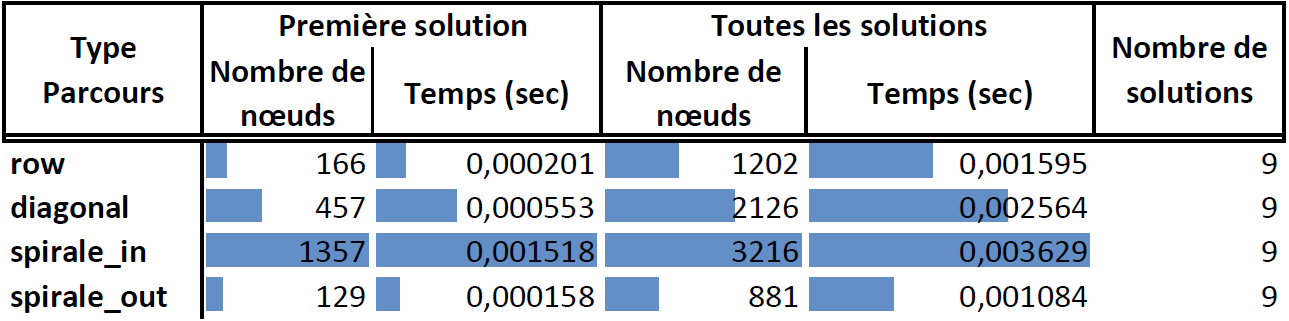
\includegraphics[width=\linewidth]{images/resultat_bruteforce_4}
		\caption{Résultats de la bruteforce pour une instance de taille 4}
	\end{table}
	\begin{table}[H]
		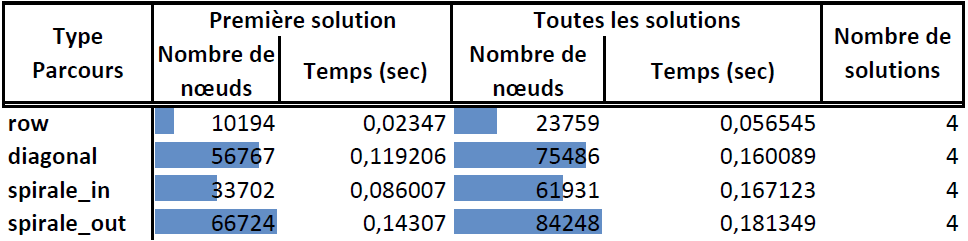
\includegraphics[width=\linewidth]{images/resultat_bruteforce_5}
		\caption{Résultats de la bruteforce pour une instance de taille 5}
	\end{table}
	\begin{table}[H]
		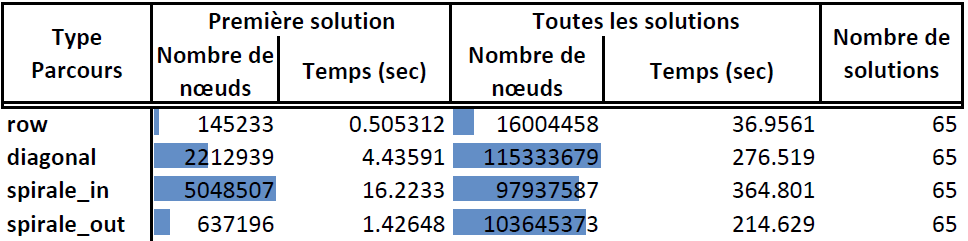
\includegraphics[width=\linewidth]{images/resultat_bruteforce_6}
		\caption{Résultats de la bruteforce pour une instance de taille 6}
	\end{table}
	
	\begin{figure}[H]
		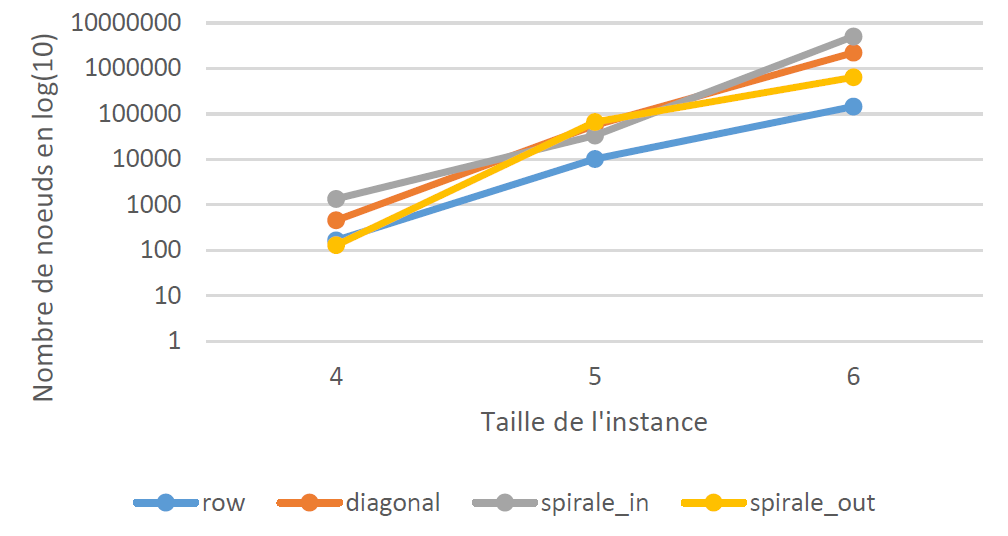
\includegraphics[width=\linewidth]{images/resultat_bruteforce_graphique_first}
		\caption{Nombre de n\oe uds à la première solution en fonction de la taille de l'instance}
		\label{fig:results_bruteforce_graphique_first}
	\end{figure}
	
	\begin{figure}[H]
		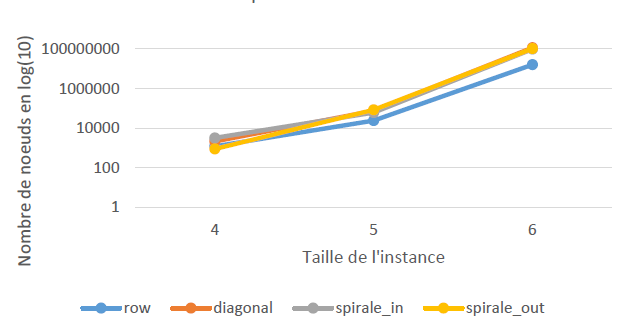
\includegraphics[width=\linewidth]{images/resultat_bruteforce_graphique_all}
		\caption{Nombre total de n\oe uds en fonction de la taille de l'instance}
		\label{fig:results_bruteforce_graphique_all}
	\end{figure}
	
	\begin{table}[H]
		\centering
		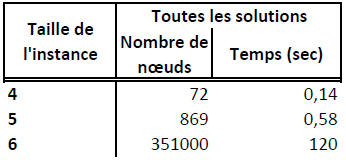
\includegraphics[width=0.6\linewidth]{images/resultat_bruteforce_rowscan_bourreau}
		\caption{Résultats de la bruteforce (rowscan) en programmation par contrainte}
	\end{table}
	
	\begin{figure}[H]
		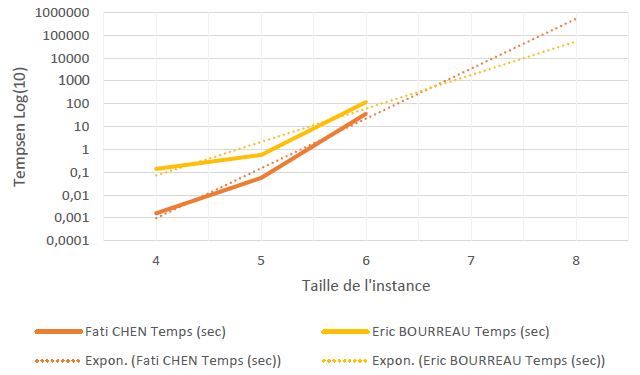
\includegraphics[width=\linewidth]{images/resultat_bruteforce_rowscan}
		\caption{Temps nécessaire au parcours complet de l'arbre}
		\label{fig:results_bruteforce_graphique_compare}
	\end{figure}

	\subsection{Smartforce}\label{annexe:smartforce}
		\begin{table}[H]
			\centering
			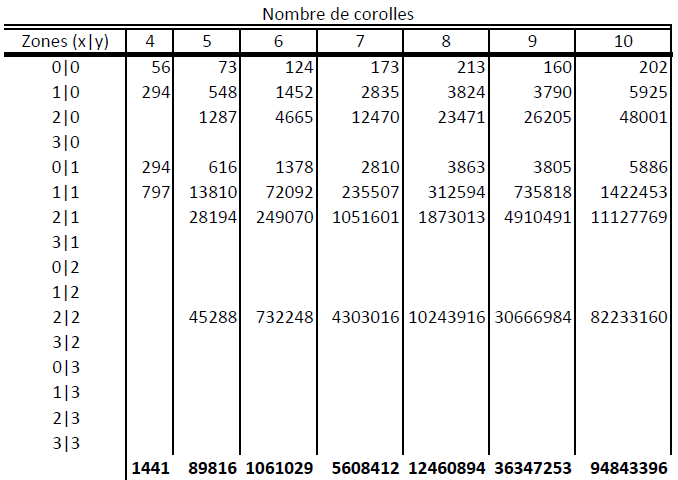
\includegraphics[width=0.8\linewidth]{images/resultats_corolle_hamming_1}
			\caption{Quantité de corolles de hamming 1 en fonction de la taille de l'instance}
		\end{table}
		
		\begin{table}[H]
			\centering
			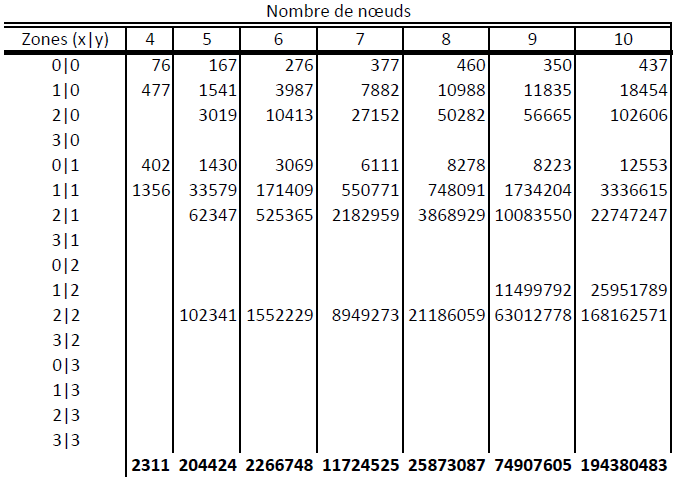
\includegraphics[width=0.8\linewidth]{images/resultats_corolle_hamming_1_noeuds}
			\caption{Nombre de n\oe uds afin de déterminer les corolles de hamming 1}
		\end{table}

		\begin{table}[H]
			\centering
			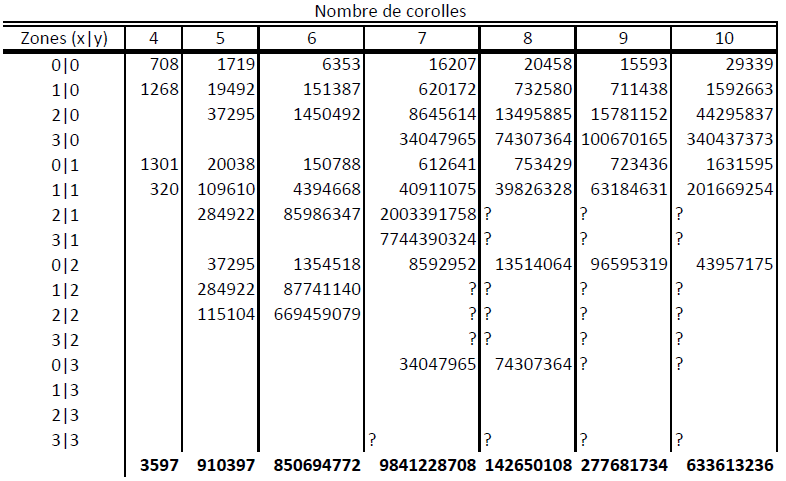
\includegraphics[width=0.8\linewidth]{images/resultats_corolle_hamming_2}
			\caption{Quantité de corolles de hamming 2 en fonction de la taille de l'instance}\label{table:count_hamming_2}
		\end{table}
		\begin{table}[H]
			\centering
			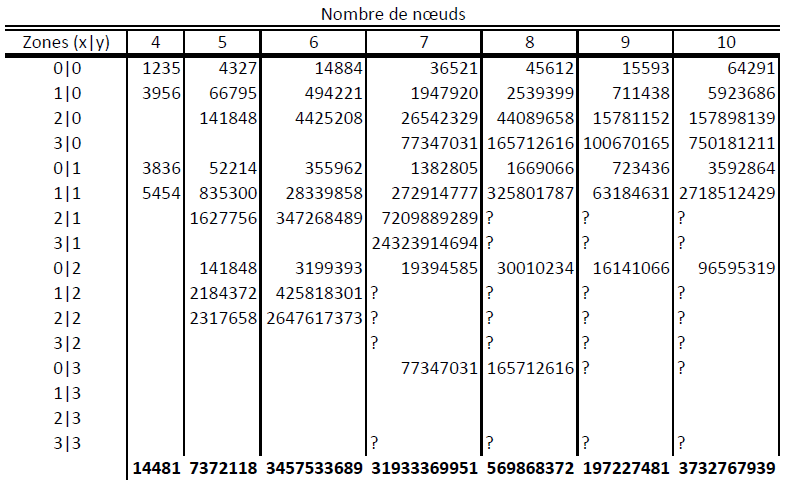
\includegraphics[width=0.8\linewidth]{images/resultats_corolle_hamming_2_noeuds}
			\caption{Nombre de n\oe uds afin de déterminer les corolles de hamming 2}
		\end{table}

	\begin{table}[H]
		\centering
		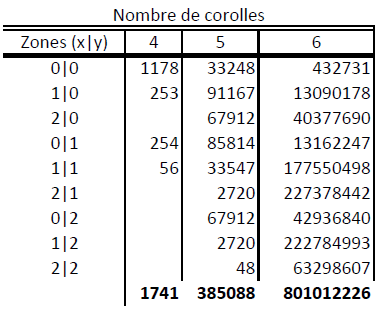
\includegraphics[width=0.6\linewidth]{images/resultats_corolle_hamming_3}
		\caption{Quantité de corolles de hamming 3 en fonction de la taille de l'instance}
	\end{table}
	\begin{table}[H]
		\centering
		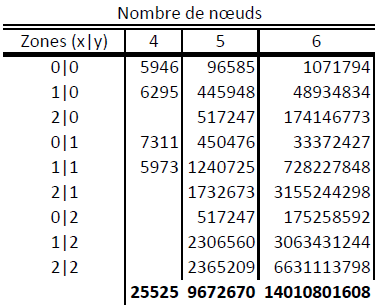
\includegraphics[width=0.6\linewidth]{images/resultats_corolle_hamming_3_noeuds}
		\caption{Nombre de n\oe uds afin de déterminer les corolles de hamming 3}
	\end{table}
\end{appendices}

	\printbibliography

\end{document}
